\documentclass[compress]{beamer}



%

\usepackage[T1]{fontenc}
%\usepackage{kmath,kerkis}
%\usepackage{fouriernc}
\usepackage[adobe-utopia]{mathdesign}
%\usepackage{arev}
\usepackage{times}
\usepackage{natbib}

\usepackage[noend]{algpseudocode}
\usepackage{xmpmulti}
\usepackage{dsfont}
\usepackage{amsmath}

\usepackage{graphicx,float,wrapfig, bbm}
\usepackage{amsfonts, comment, bbold}
\usepackage{mdwlist}
\usepackage{subfigure}
\usepackage{colortbl}
\usepackage{mathrsfs}


\usepackage{multirow}




% packages

\usepackage{amsfonts}

% environments

\newenvironment{packed_enumerate}{
  \begin{enumerate}
    \setlength{\topsep}{0pt}
    \setlength{\itemsep}{2pt}
    \setlength{\parskip}{0pt}
    \setlength{\parsep}{0pt}
}{\end{enumerate}}

\newenvironment{stepit}
 {\begin{itemize}[<+-|alert@+>]}
   {\end{itemize}}

% commands

\newcommand{\Norm}[3]{\mathcal{N}\left( #1, #2, #3 \right)}
\newcommand{\popshow}[2]{\only<#1->{\alert<#1>{#2}}}
\newcommand{\x}{\mathbf{x}}
\newcommand{\ex}[1]{\mbox{exp}\left\{ #1\right\} }
\newcommand{\e}[2]{\mathbb{E}_{#1}\left[ #2 \right] }
\newcommand{\g}{\, | \,}
\newcommand{\indpt}{\protect\mathpalette{\protect\independenT}{\perp}}
\def\independenT#1#2{\mathrel{\rlap{$#1#2$}\mkern2mu{#1#2}}}
\newcommand{\E}{\textrm{E}}
\newcommand{\R}{\textrm{R}}
\newcommand{\realline}{\mathbb{R}}
\newcommand{\data}{{\cal D}}
\newcommand{\loglik}{{\cal L}}
\newcommand{\grad}[2]{ \frac{\partial{#1}}{\partial#2}}
\newcommand{\dir}[1]{\mbox{Dir}(#1)}
\newcommand{\mult}[1]{\mbox{Mult}( #1)}
\newcommand{\G}[1]{\Gamma \left( \textstyle #1 \right)}
\newcommand{\ind}[1]{\mathds{1}\left[ #1 \right] }
\newcommand{\norm}[1]{\left\lVert#1\right\rVert}

\newcommand{\class}[1]{ \texttt{#1}}
\newcommand{\term}[1]{ ``#1''}
\newcommand{\tcword}[0]{ w }
\newcommand{\docsetlabeled}[0]{ D }
\newcommand{\onedoclabeled}[0]{ d }
\newcommand{\tcposindex}[0]{ i }
\newcommand{\myblue}[1]{ {\textbf #1 }}
\newcommand{\dnrm}[1]{ _{\mbox{\textsc{ #1 }}}}
\newcommand{\argmax}[0]{ \arg \max }
\newcommand{\tcjclass}[0]{c_j}
\newcommand{\maths}[1]{ {\bf #1}}




% complexity
\renewcommand{\O}{\mathcal{O}}



\setbeamersize{text margin left=0.5cm}
\setbeamersize{text margin right=0.5cm}
\setbeamercolor{alert}{fg=red!75!black}

\usetheme{default}
\useinnertheme{circles}
\useoutertheme{split}
\usecolortheme{seahorse}
% \usecolortheme{dove}
% \usecolortheme{seagull}
%\usecolortheme{default}
% \usecolortheme{dolphin}
\usefonttheme{structurebold}
%\usefonttheme{serif}

\setbeamertemplate{navigation symbols}{}
\setbeamertemplate{headline}{}
\setbeamertemplate{footline}{}
\setbeamerfont{itemize/enumerate subbody}{size=\normalsize}
\setbeamerfont{itemize/enumerate subsubbody}{size=\normalsize}
\setbeamercolor{itemize item}{fg=gray}
\setbeamercolor{enumerate item}{fg=gray}
\setbeamercolor{itemize item}{fg=gray}
\setbeamercolor{itemize subitem}{fg=gray}
\setbeamercolor{item projected}{bg=gray}
\setbeamercolor{subitem projected}{bg=gray}


\newenvironment{bullets}
{\begin{itemize} \setlength{\itemsep}{10pt}}
{\end{itemize}}

\newcommand{\mygraphic}[2]{
  \begin{beamercolorbox}[colorsep*=4pt]{black math}
    \begin{center}
      \includegraphics[#1]{#2}
    \end{center}
  \end{beamercolorbox}
}

\setbeamercolor{structure}{bg=gray}
\setbeamercolor{section in head/foot}{bg=gray}
\setbeamercolor{palette primary}{bg=lightgray}


\usepackage{minted}

\usetheme[pageofpages=of,                    % String used between the current page and the
                                             % total page count.
          bullet=circle,                     % Use circles instead of squares for bullets.
          titleline=true,                    % Show a line below the frame title.
          showdate=true,                     % show the date on the title page
          alternativetitlepage=true,         % Use the fancy title page.
          titlepagelogo=../../common/culogo,              % Logo for the first page.
          % Logo for the header on first page.
          headerlogo=../../common/boulder_cs,
          ]{UCBoulder}

\usecolortheme{ucdblack}
\author{Introduction to Data Science Algorithms}


\institute[Boyd-Graber and Paul] % (optional, but mostly needed)
{Jordan Boyd-Graber and Michael Paul}


\AtBeginSection[] % "Beamer, do the following at the start of every section"
{ \begin{frame} \frametitle{Outline} % make a frame titled "Outline"
\tableofcontents[currentsection] % show TOC and highlight current section
\end{frame} }


\usepackage{tikz-dependency}
%\usepackage{tikz-qtree}
\usepackage{qtree}
\usepackage{pdfpages}

\newcommand{\gfx}[2]{
\begin{center}
	\includegraphics[width=#2\linewidth]{distsim/#1}
\end{center}
}
\title{Distributional Semantics}
\date{Slides Adapted from Yoav Goldberg and Omer Levy}

\begin{document}

\tikzstyle{every picture}+=[remember picture]



\begin{frame}
  \titlepage
\end{frame}


\begin{frame}{From Distributional to Distributed Semantics}
    \begin{block}{The new kid on the block}
        \begin{itemize}
            \item Deep learning / neural networks
            \item ``Distributed'' word representations
                \begin{itemize}
                    \item Feed text into neural-net. Get back ``word
                        embeddings''.
                    \item Each word is represented as a low-dimensional vector.
                    \item Vectors capture ``semantics''
                \end{itemize}
            \item \texttt{word2vec} (Mikolov et al)
        \end{itemize}
    \end{block}
\end{frame}

\begin{frame}{From Distributional to Distributed Semantics}
    \begin{block}{This part of the talk}
        \begin{itemize}
            \item \texttt{word2vec} as a black box
            \item a peek inside the black box
            \item relation between word-embeddings and the distributional
                representation
            \item tailoring word embeddings to your needs using
                \texttt{word2vec}
        \end{itemize}
    \end{block}
\end{frame}

\begin{frame}{word2vec}

    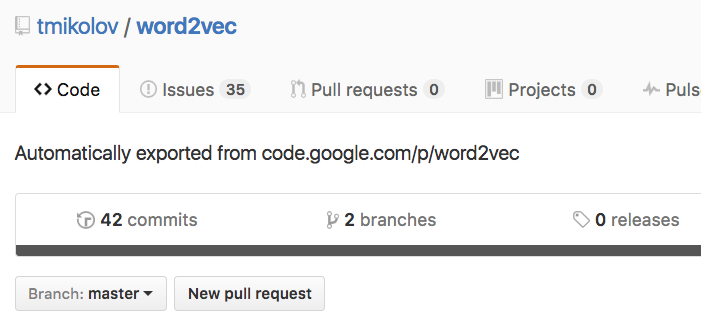
\includegraphics[width=\textwidth]{distsim/word2vec_site}

\end{frame}

\begin{frame}{word2vec}

    \centering
    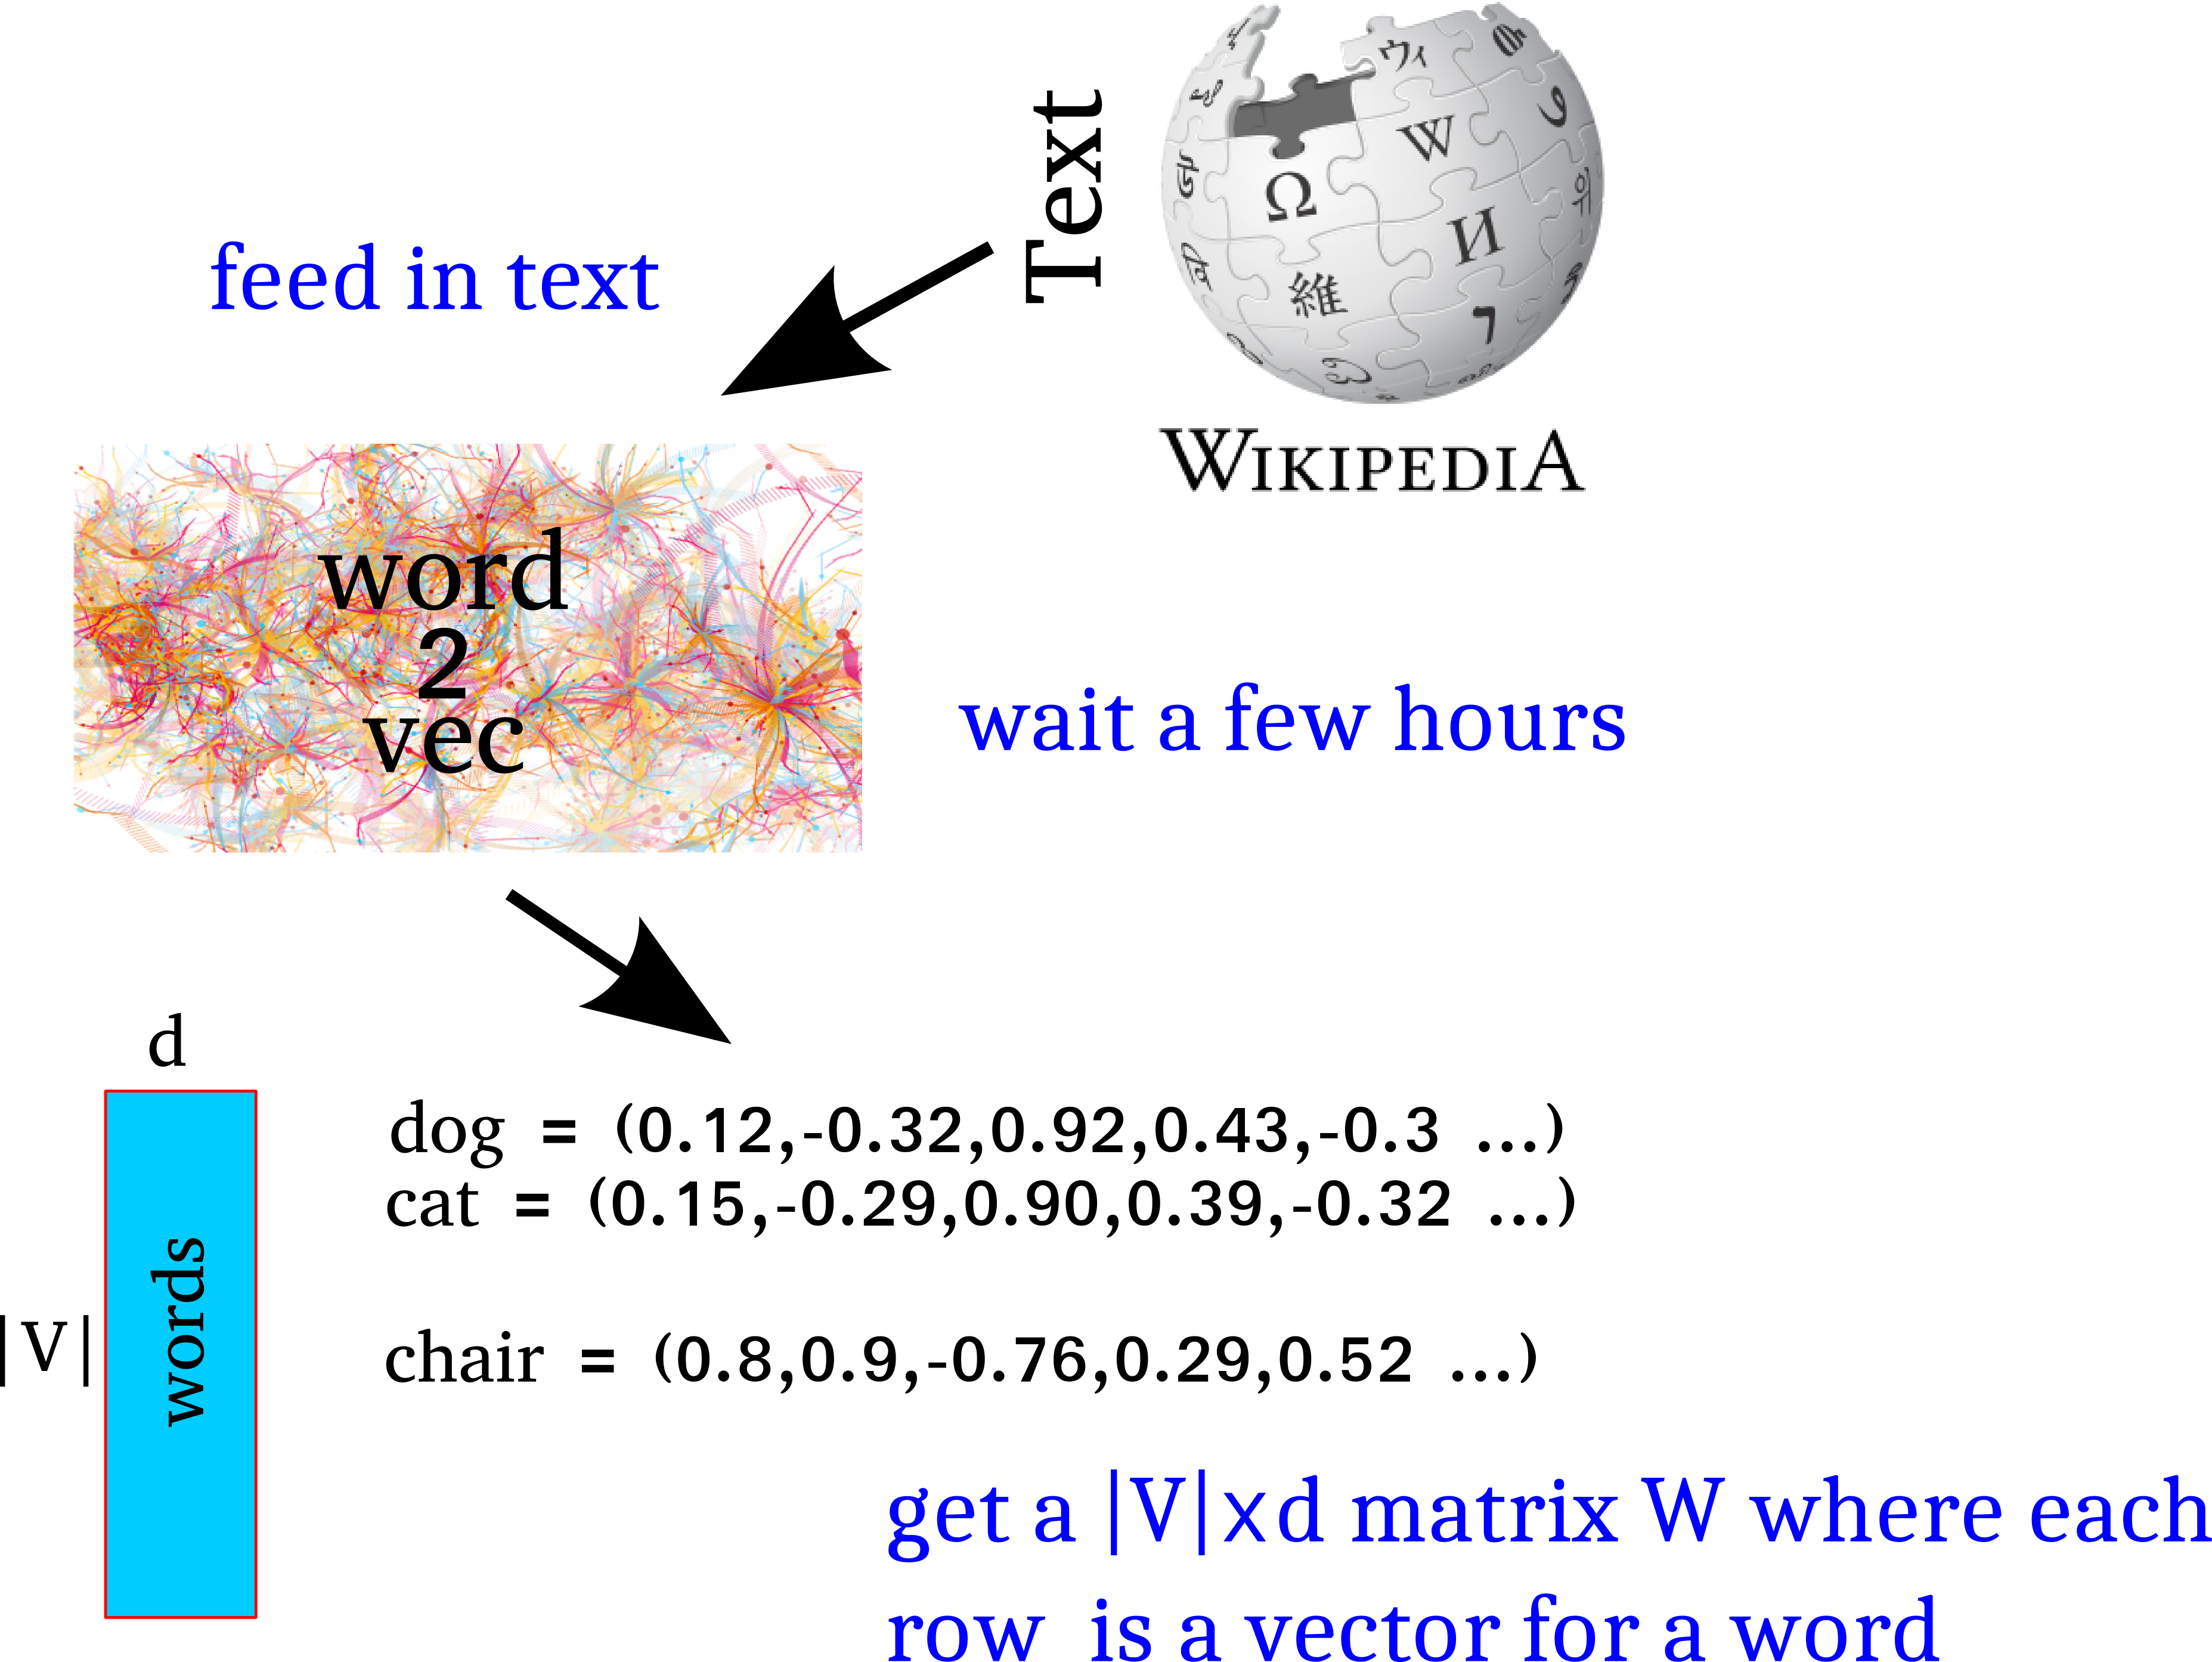
\includegraphics[width=0.8\textwidth]{distsim/w2v_flow.png}

\end{frame}

\begin{frame}{word2vec}

    \begin{itemize}
        \item dog
            \begin{itemize}
                \item cat, dogs, dachshund, rabbit, puppy, poodle, rottweiler,
                    mixed-breed, doberman, pig
            \end{itemize}
        \item sheep
            \begin{itemize}
                \item cattle, goats, cows, chickens, sheeps, hogs, donkeys,
                    herds, shorthorn, livestock
            \end{itemize}
        \item november
            \begin{itemize}
                \item october, december, april, june, february, july, september,
                    january, august, march
            \end{itemize}
        \item jerusalem
            \begin{itemize}
                \item tiberias, jaffa, haifa, israel, palestine, nablus, damascus
                    katamon, ramla, safed
            \end{itemize}
        \item teva
            \begin{itemize}
                \item pfizer, schering-plough, novartis, astrazeneca,
                    glaxosmithkline, sanofi-aventis, mylan, sanofi, genzyme, pharmacia
            \end{itemize}
    \end{itemize}
\end{frame}


\begin{frame}{Working with Dense Vectors}

    \begin{block}{Word Similarity}
        \begin{itemize}
            \item Similarity is calculated using \textit{cosine
                similarity}:
        \end{itemize}
        \[sim(\vec{dog}, \vec{cat}) = \frac{\vec{dog} \cdot \vec{cat}}{||\vec{dog}|| \; ||\vec{cat}||}\]
        \begin{itemize}
            \item For normalized vectors ($||x|| = 1$), this is equivalent to a
                dot product:
        \end{itemize}
        \[sim(\vec{dog}, \vec{cat}) = \vec{dog} \cdot \vec{cat}\]
        \begin{itemize}
            \item \textbf{Normalize the vectors when loading them.}
        \end{itemize}
    \end{block}


\end{frame}

\begin{frame}[fragile]{Working with Dense Vectors}
    \begin{block}{Finding the most similar words to $\vec{dog}$}
        \begin{itemize}
            \item Compute the similarity from word $\vec{v}$ to all other words.
                \pause
            \item This is a \textbf{single matrix-vector product}: $W \cdot \vec{v}^\top$
                \begin{center}
                    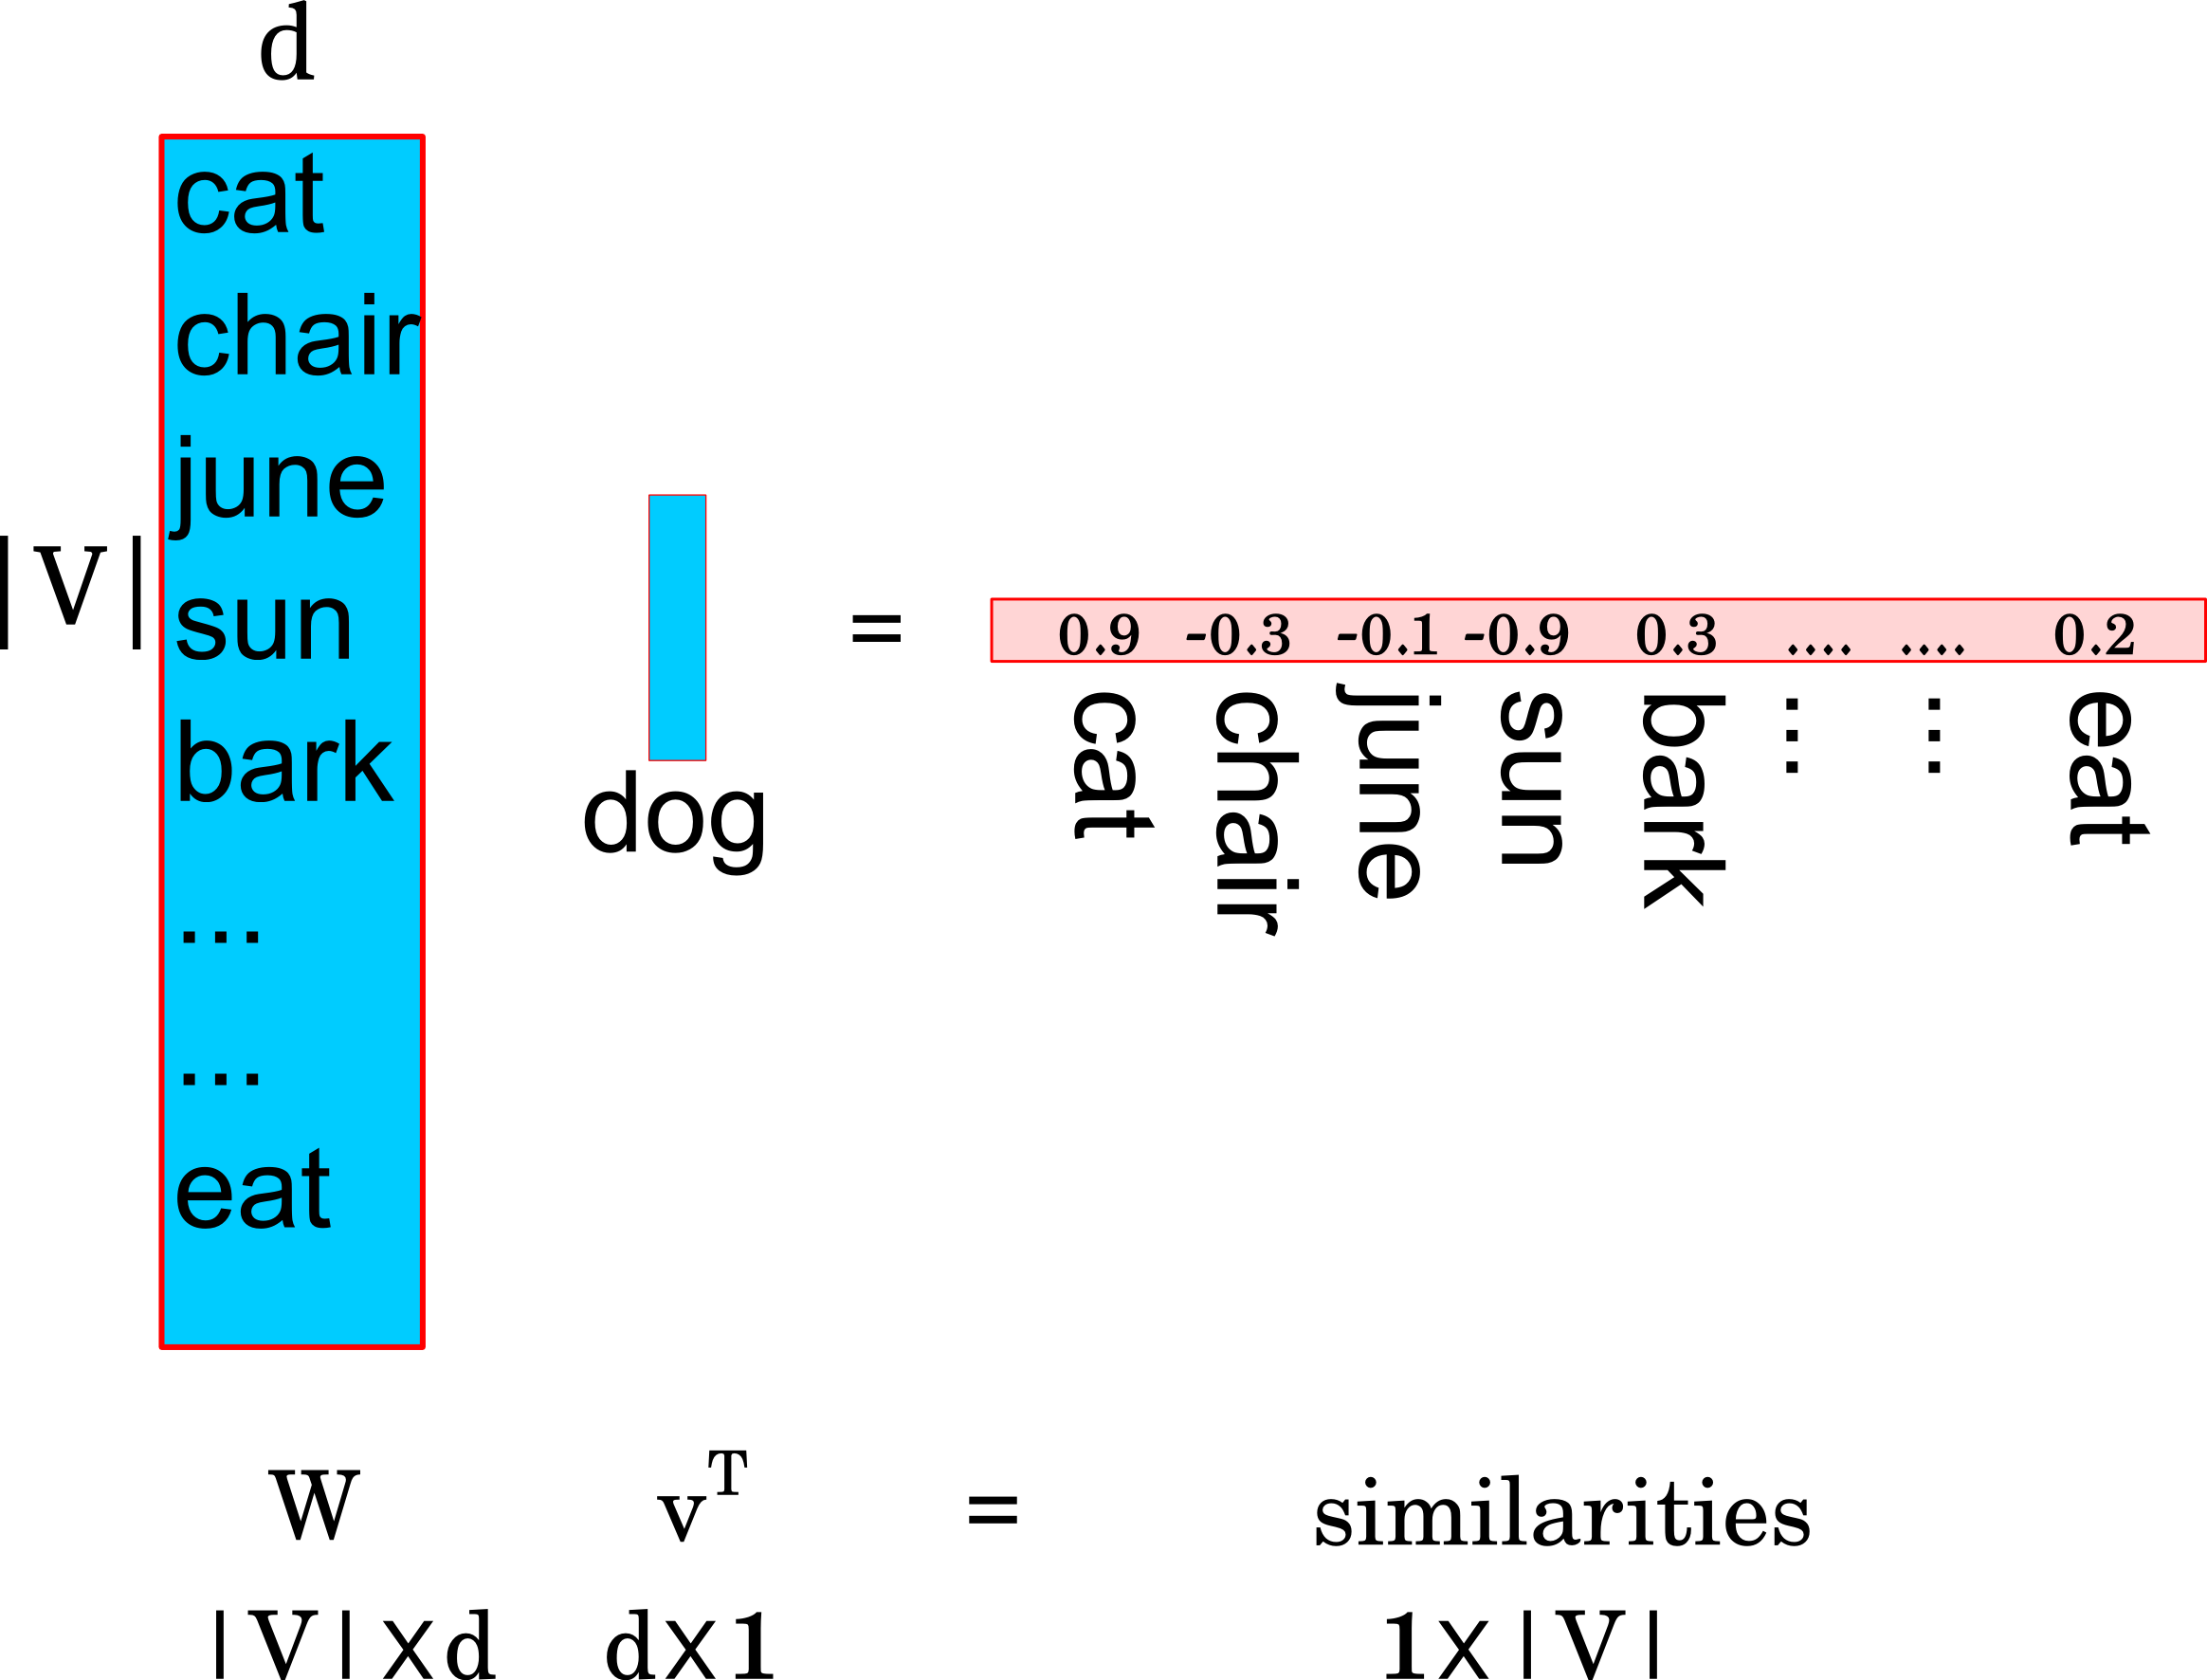
\includegraphics[width=0.4\textwidth]{distsim/Wv.png}
                \end{center}
                \pause
            \item Result is a $|V|$ sized vector of similarities.
            \item Take the indices of the $k$-highest values.
                \pause
            \item \textbf{FAST! for 180k words, d=300: $\sim$30ms}
        \end{itemize}
    \end{block}
\end{frame}

\begin{frame}[fragile]{Working with Dense Vectors}
    \begin{block}{Most Similar Words, in python+numpy code}
   \begin{minted}{python}
W,words = load_and_norm_vectors("vecs.txt")
# W and words are numpy arrays.
w2i = {w:i for i,w in enumerate(words)}

dog = W[w2i['dog']] # get the dog vector

sims = W.dot(dog)   # compute similarities

most_similar_ids = sims.argsort()[-1:-10:-1]
sim_words = words[most_similar_ids]
   \end{minted}
   \end{block}
\end{frame}

\begin{frame}[fragile]{Working with Dense Vectors}
    \begin{block}{Similarity to a group of words}
        \begin{itemize}
            \item ``Find me words most similar to cat, dog and cow''.
            \item Calculate the pairwise similarities and sum them:
                \[W \cdot \vec{cat} + W \cdot \vec{dog} + W \cdot \vec{cow} \]
            \item Now find the indices of the highest values as before.
                \pause
        \end{itemize}
        \begin{itemize}
            \item Matrix-vector products are wasteful. \textbf{Better option:}
                \[W \cdot (\vec{cat} + \vec{dog} + \vec{cow}) \]
        \end{itemize}
    \end{block}
\end{frame}

\begin{frame}{}

    \centering
    Working with dense word vectors can be very efficient.

    \vspace{2em}

    \pause
    But where do these vectors come from?

\end{frame}

\begin{frame}{How does word2vec work?}

    word2vec implements several different algorithms:

    \begin{block}{Two training methods}
    \begin{itemize}
        \item \textbf<2>{Negative Sampling}
        \item Hierarchical Softmax
    \end{itemize}
    \end{block}
    \begin{block}{Two context representations}
    \begin{itemize}
        \item Continuous Bag of Words (CBOW)
        \item \textbf<2>{Skip-grams}
    \end{itemize}
    \end{block}

    \pause
    \vspace{1em}
    We'll focus on skip-grams with negative sampling

    \vspace{1em}
    intuitions apply for other models as well
\end{frame}

\begin{frame}{How does word2vec work?}
    \begin{itemize}
        \item Represent each word as a $d$ dimensional vector.
        \item Represent each context as a $d$ dimensional vector.
        \item Initalize all vectors to random weights.
        \item Arrange vectors in two matrices, $W$ and $C$.
    \end{itemize}
    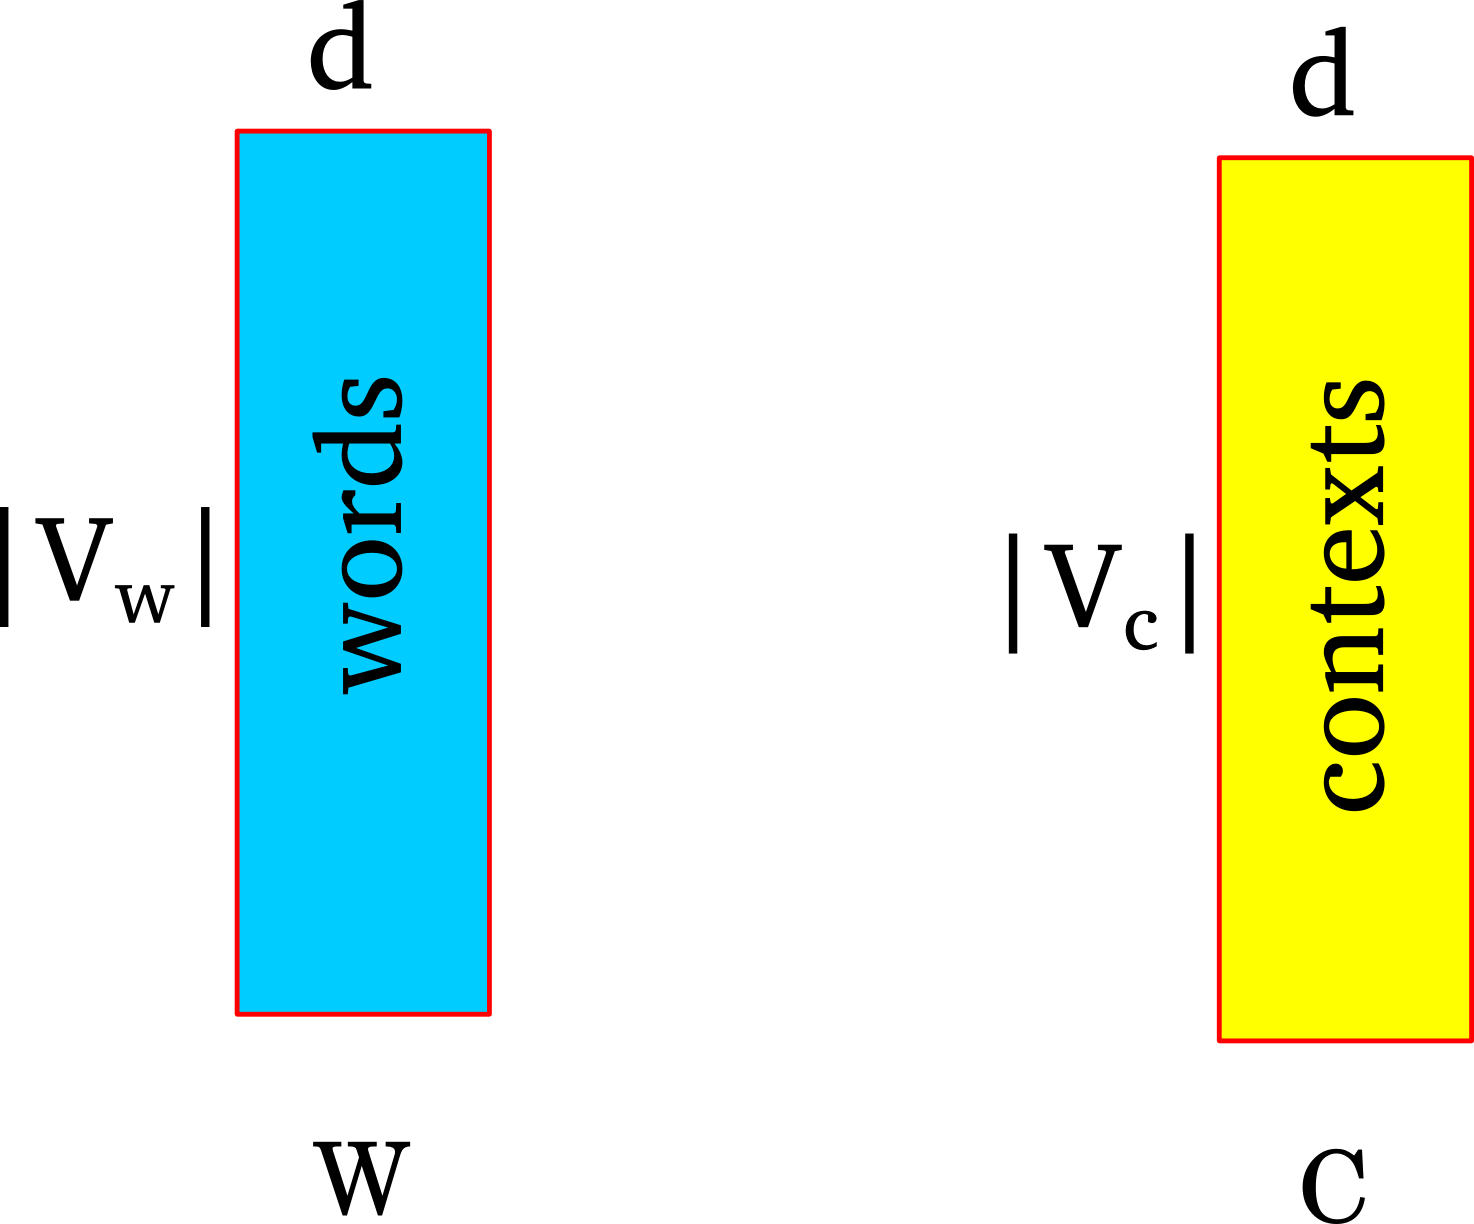
\includegraphics[width=0.5\textwidth]{distsim/WC.png}
\end{frame}

\begin{frame}{How does word2vec work?}
    While more text:
    \begin{itemize}
        \item Extract a word window:
    \end{itemize}
    \scalebox{0.8}{
\begin{tabular}{ccccccccc}
\texttt{A springer is} [ & \texttt{a}     & \texttt{cow}   & \texttt{or}
& \texttt{\textbf{heifer}} & \texttt{close} & \texttt{to} &
\texttt{calving} & ] \texttt{.} \\
          & $c_1$ & $c_2$ & $c_3$ & $w$            &  $c_4$ & $c_5$  & $c_6$ &  \\
      \end{tabular}}
      \only<1>{
      \begin{itemize}
          \item $w$ is the focus word vector (row in $W$).
          \item $c_i$ are the context word vectors (rows in $C$).
      \end{itemize}
        }

        \pause
    \begin{itemize}
        \item Try setting the vector values such that:
            \[\sigma(w\cdot~c_1) + \sigma(w\cdot~c_2) + \sigma(w\cdot~c_3) +
            \sigma(w\cdot~c_4) + \sigma(w\cdot~c_5) + \sigma(w\cdot~c_6)\]
            is \textbf{high}
    \end{itemize}
        \pause
    \begin{itemize}
        \item Create a corrupt example by choosing a random word $w'$
        \scalebox{0.8}{
    \begin{tabular}{ccccccccc}
    [ & \texttt{a}     & \texttt{cow}   & \texttt{or}
    & \texttt{\textbf{comet}} & \texttt{close} & \texttt{to} &
    \texttt{calving} & ] \\
              & $c_1$ & $c_2$ & $c_3$ & $w'$            &  $c_4$ & $c_5$  & $c_6$ &  \\
          \end{tabular}}
    \end{itemize}

    \begin{itemize}
        \item Try setting the vector values such that:
            \[\sigma(w'\cdot~c_1) + \sigma(w'\cdot~c_2) + \sigma(w'\cdot~c_3) +
            \sigma(w'\cdot~c_4) + \sigma(w'\cdot~c_5) + \sigma(w'\cdot~c_6)\]
            is \textbf{low}
    \end{itemize}
\end{frame}

\begin{frame}{How does word2vec work?}

    The training procedure results in:
    \begin{itemize}
        \item $w\cdot c$ for \textbf{good} word-context pairs is \textbf{high}
        \item $w\cdot c$ for \textbf{bad} word-context pairs is \textbf{low}
        \item $w\cdot c$ for \textbf{ok-ish} word-context pairs is \textbf{neither high nor low}
    \end{itemize}

    \vspace{1em}
    As a result:
    \begin{itemize}
        \item Words that share many contexts get close to each other.
        \item Contexts that share many words get close to each other.
    \end{itemize}

    \vspace{1em}
    At the end, word2vec throws away $C$ and returns $W$.



\end{frame}

\begin{frame}{Reinterpretation}

    Imagine we didn't throw away $C$. Consider the product $WC^\top$
    \pause
    \vspace{1em}

    \begin{center}
    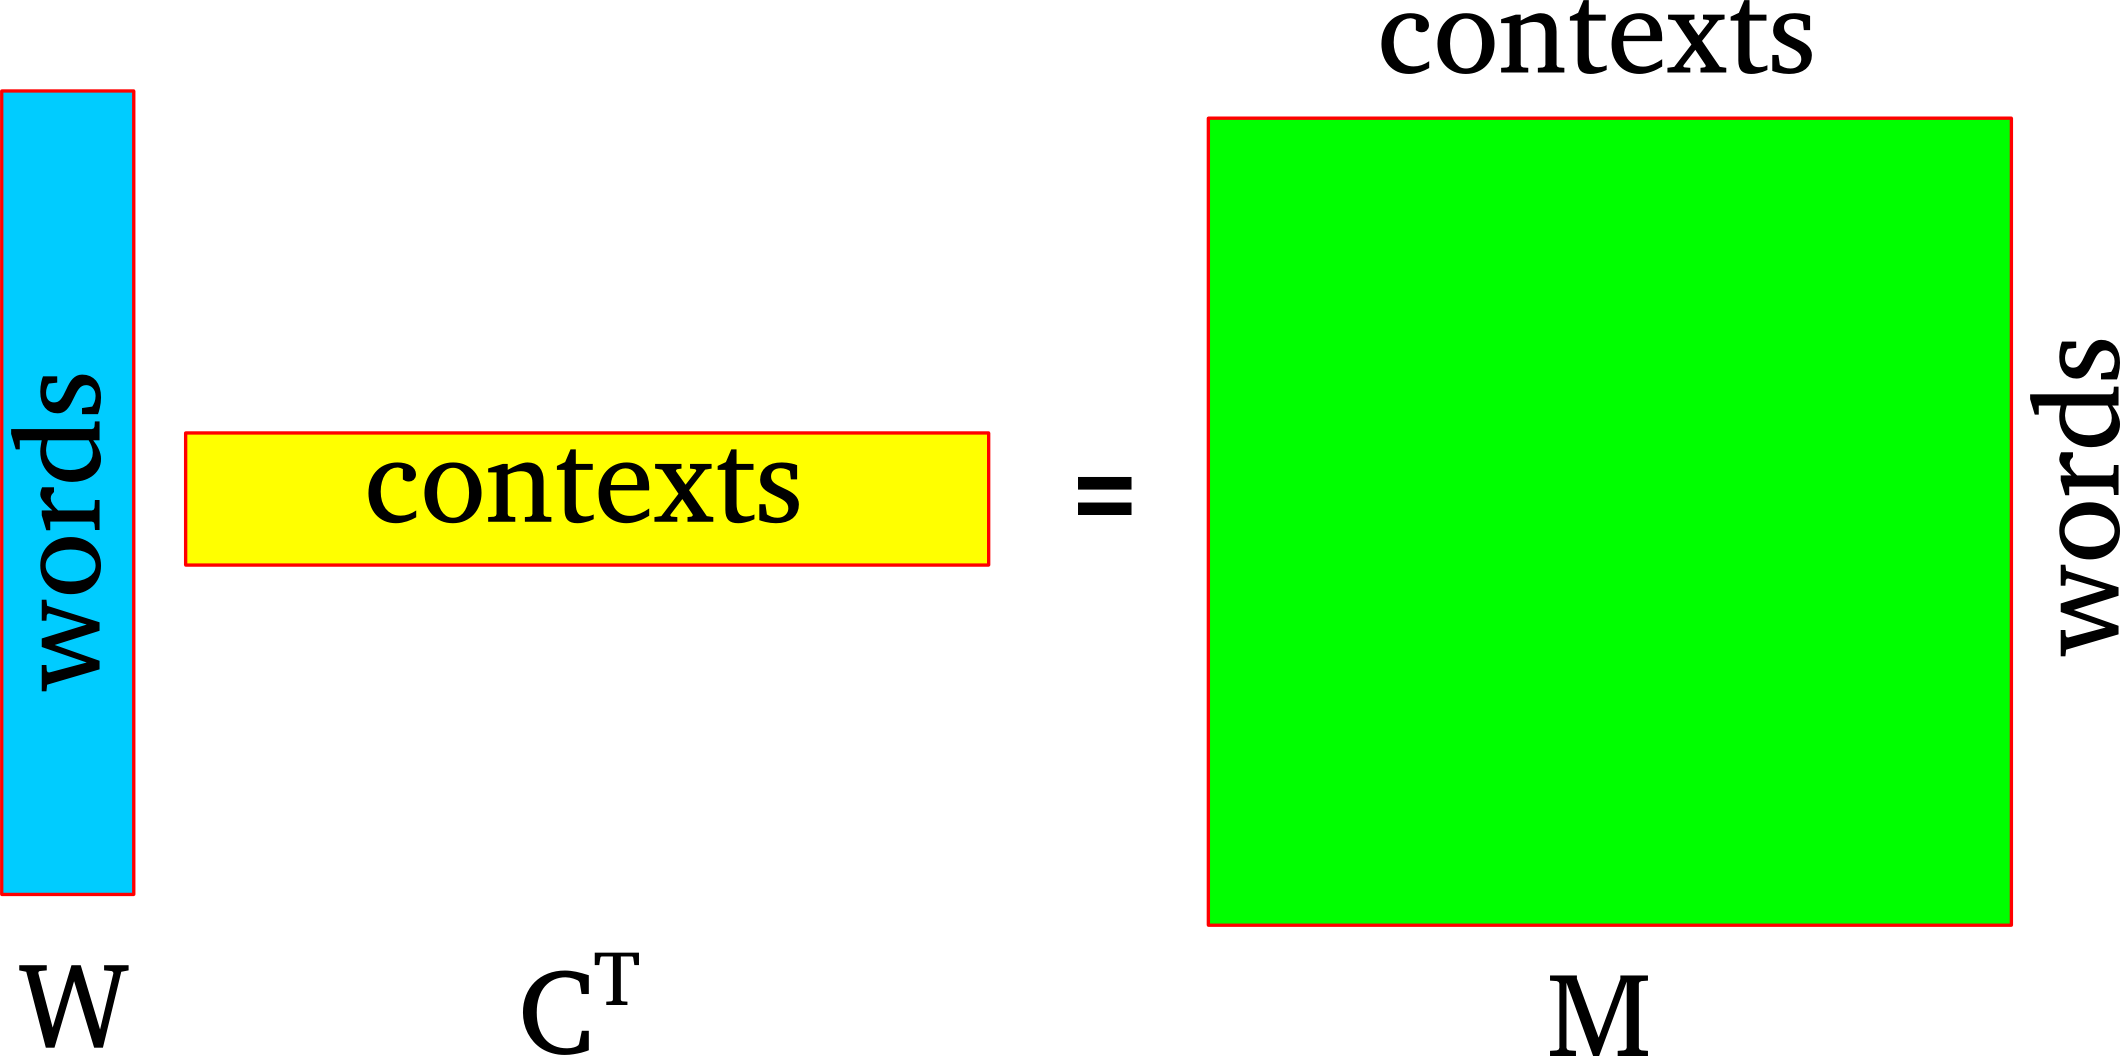
\includegraphics[width=0.6\textwidth]{distsim/word_context_matrix.png}
    \end{center}

    \vspace{1em}
    The result is a matrix $M$ in which:
    \begin{itemize}
        \item Each row corresponds to a word.
        \item Each column corresponds to a context.
        \item Each cell: $w\cdot c$, association between
            word and context.
    \end{itemize}

\end{frame}

\begin{frame}{Reinterpretation}

    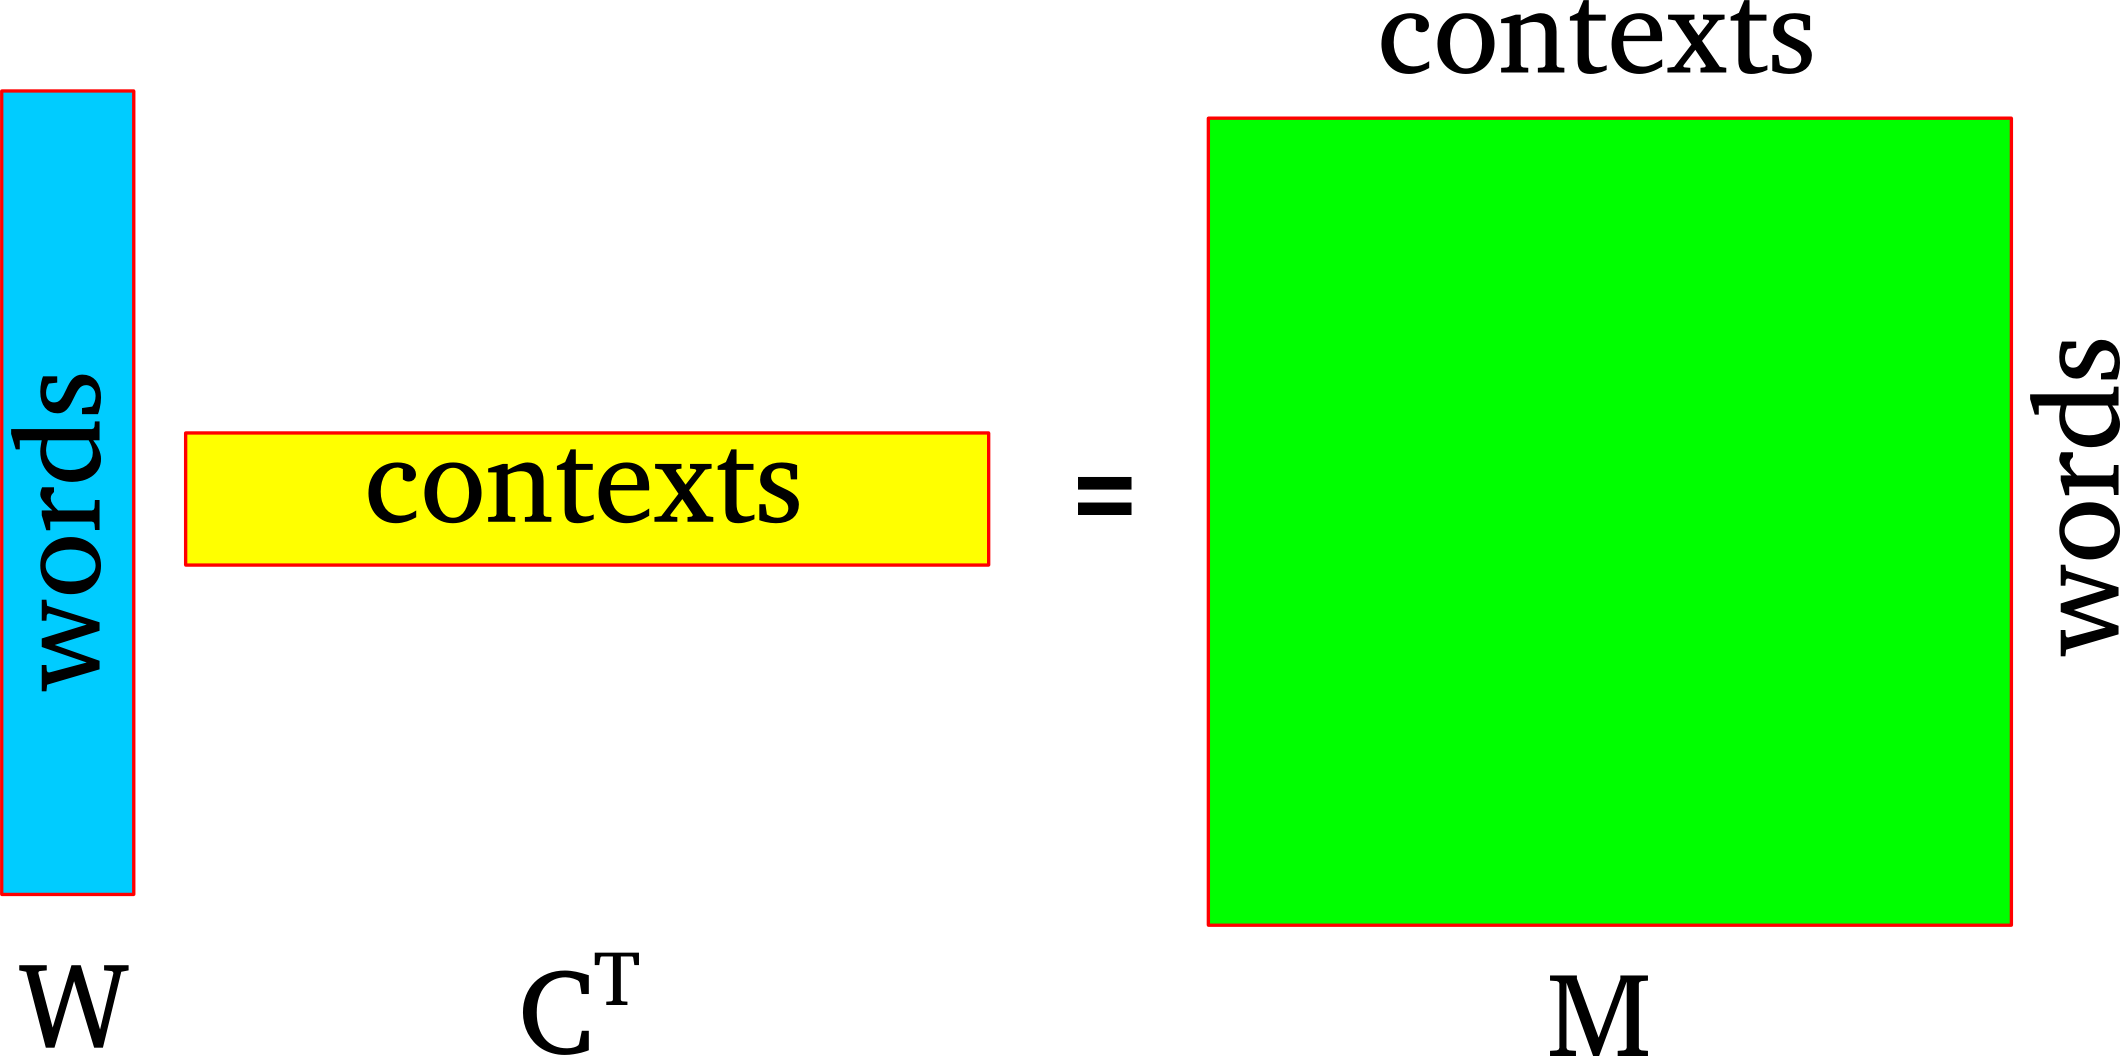
\includegraphics[width=0.5\textwidth]{distsim/word_context_matrix.png}

    \vspace{1em}
    Does this remind you of something?
    \pause

    \vspace{0.3em}
    Very similar to SVD over distributional representation:
    \vspace{1em}

    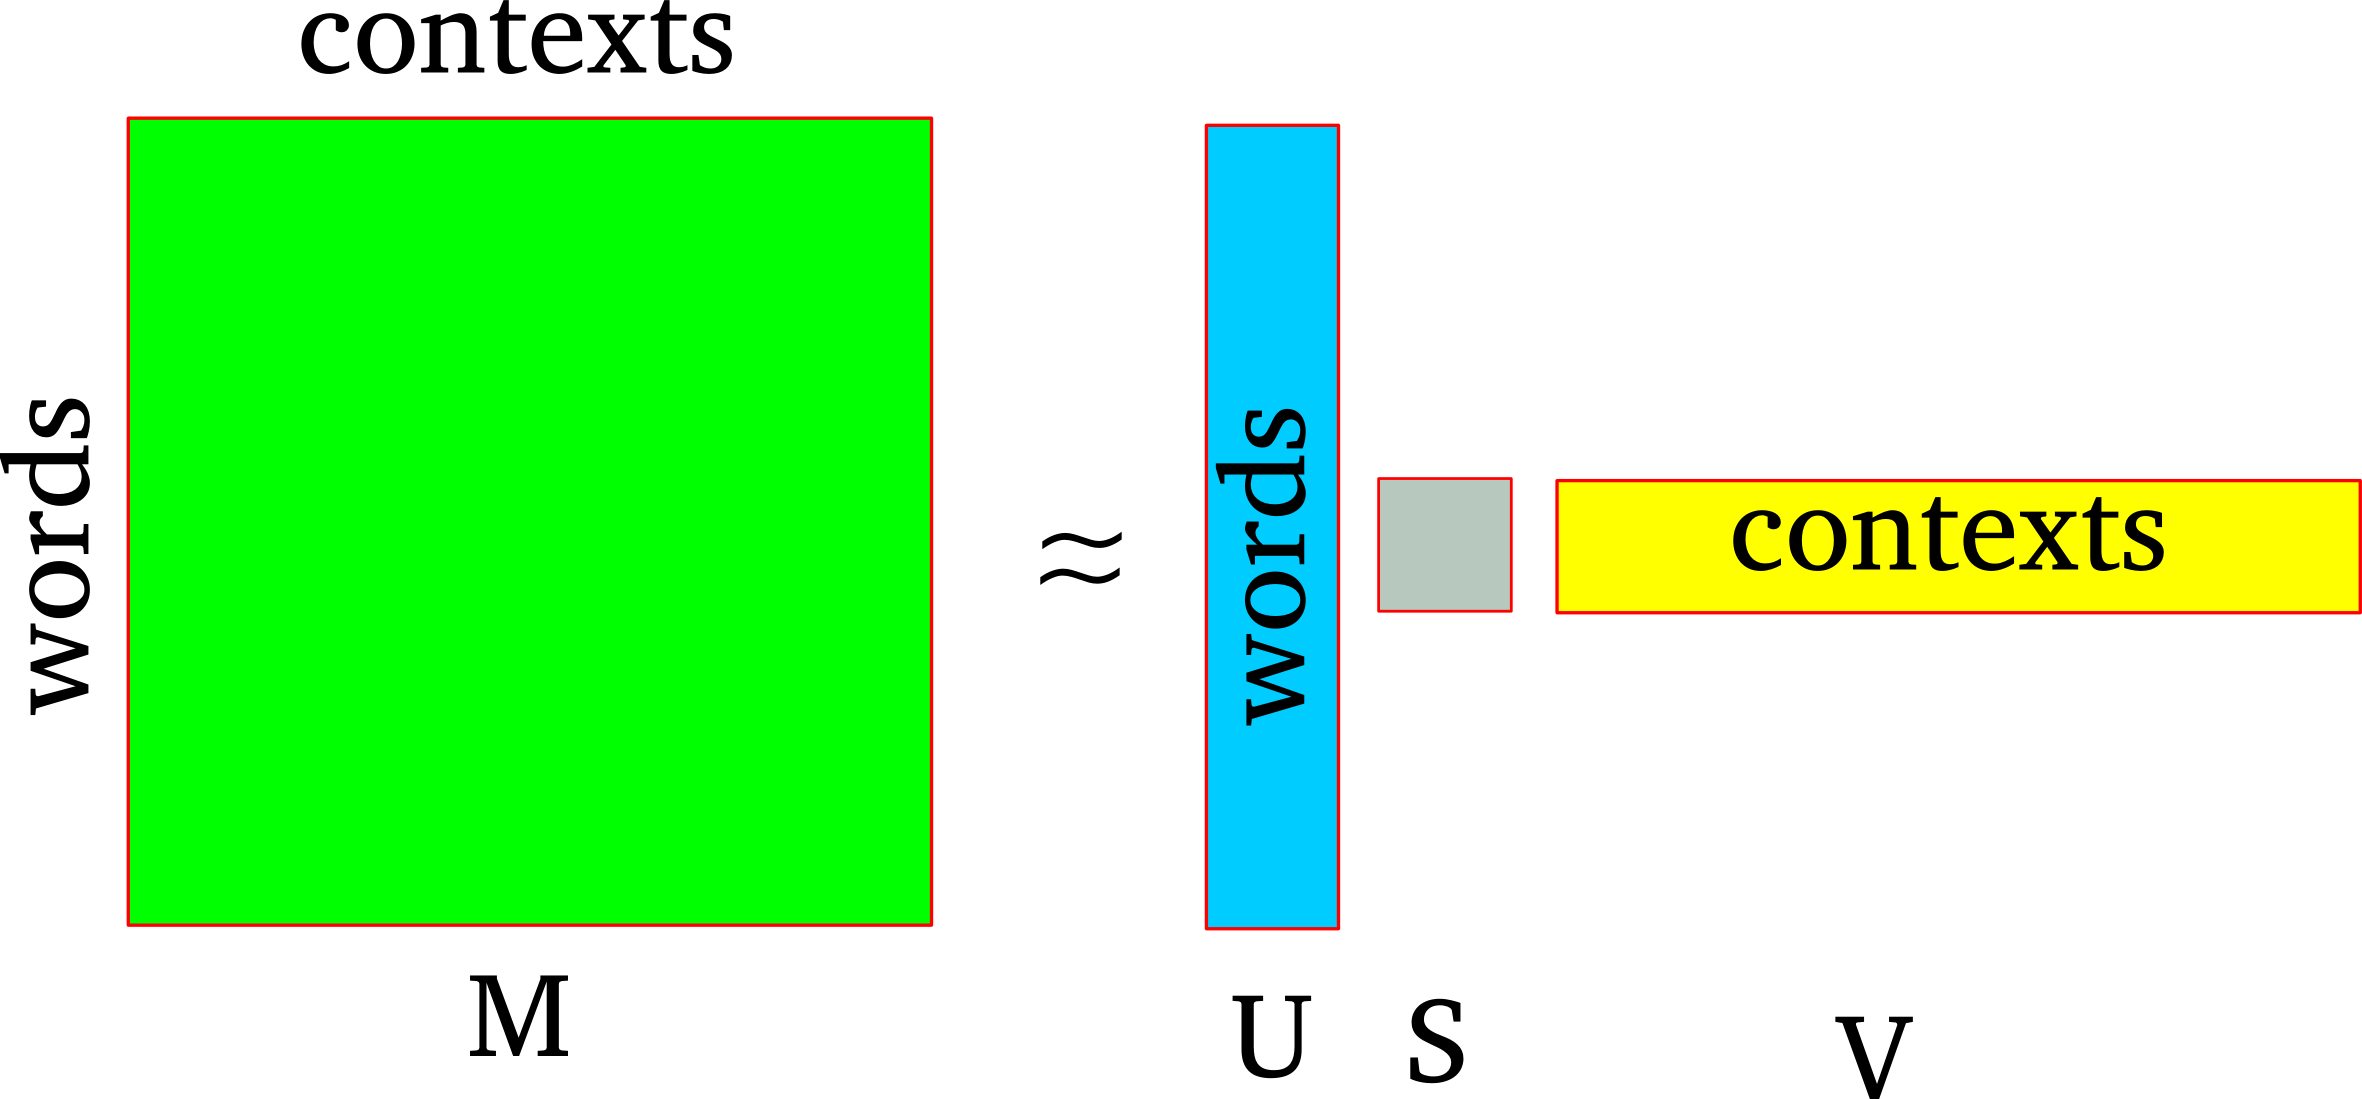
\includegraphics[width=0.5\textwidth]{distsim/svd.png}

\end{frame}

\begin{frame}{Relation between SVD and word2vec}
    \begin{block}{SVD}
        \begin{itemize}
            \item Begin with a word-context matrix.
            \item Approximate it with a product of low rank (thin) matrices.
            \item Use thin matrix as word representation.
        \end{itemize}
    \end{block}
    \begin{block}{\texttt{word2vec} (skip-grams, negative sampling)}
        \begin{itemize}
            \item Learn thin word and context matrices.
            \item These matrices can be thought of as approximating an implicit word-context
                matrix.
                \begin{itemize}
                    \item Levy and Goldberg (NIPS 2014) show that this
                        implicit matrix is related to the well-known PPMI matrix.
                \end{itemize}
        \end{itemize}
    \end{block}
\end{frame}

\begin{frame}{Relation between SVD and word2vec}
word2vec is a dimensionality reduction technique over an (implicit) word-context
matrix.

\vspace{1em}

Just like SVD.

\vspace{1em}
With few tricks {\footnotesize(Levy, Goldberg and Dagan, TACL 2015)}
we can get SVD to perform just as well as \texttt{word2vec}.

\pause
\vspace{1em}
However, \texttt{word2vec}\ldots

\begin{itemize}
    \item \textbf{\ldots works without building / storing the actual matrix in memory.}
    \item \textbf{\ldots is very fast to train, can use multiple threads.}
    \item \textbf{\ldots can easily scale to huge data and very large word
and context vocabularies.}
\end{itemize}
\end{frame}

%\begin{frame}{word2vec vs. distributional}
%    @@ TODO: remove / move this slide? @@
%    \begin{block}{When should we consider the sparse distributional representation?}
%        \begin{itemize}
%            \item Relatively small amounts of data.
%            \item The input comes as counted word-context pairs.
%            \item Want to interpret the different dimensions.
%            \item Want a more complex similarity measure, i.e. directional
%                similarity.
%        \end{itemize}
%    \end{block}
%\end{frame}

\end{document}